\chapter{Data Compression}
In this chapter we investigate how a given string can be stored so that the amount of memory used to store the
string is minimized.   We assume that a set of characters $\Sigma$ is given and that the string $s$ is a finite
sequence of characters from $\Sigma$, i.e.~$s \in \Sigma^*$.  The set of characters $\Sigma$ is called the
\blue{alphabet}.  If the alphabet $\Sigma$ contains $k$ different characters and if we use the same number of
bits $b$ for every character in $\Sigma$, then the number $b$ of bits must satisfy the inequality
\\[0.2cm]
\hspace*{1.3cm}
$\ds k \leq 2^b$,
\\[0.2cm]
which entails that 
\\[0.2cm]
\hspace*{1.3cm}
$b \geq \mytt{ceil}\bigl(\log_2(k)\bigr)$
\\[0.2cm]
holds.  Here, $\mytt{ceil}(x)$ denotes the
\href{https://en.wikipedia.org/wiki/Floor_and_ceiling_functions}{ceiling function}.  Given a real number $x$,
the expression $\mytt{ceil}(x)$ returns the smallest integer $k$ that is as least as big as $x$, i.e.~we have
\\[0.2cm]
\hspace*{1.3cm}
$\mytt{ceil}(x) = \min \{ k \in \mathbb{Z} \mid x \leq k \}$. 
\\[0.2cm]
If the string $s$ has a length of $m$ characters, then we have to use $m \cdot b$ bits in order to code $s$. 
There are two options to improve on this number.
\begin{enumerate}
\item If we drop the requirement to store all characters with the same amount of bits, then we can save some space.
      The idea is to code characters occurring very frequently with fewer than $b$ bits while those characters
      that are very rare are encoded using more than $b$ bits.  This approach leads to 
      \href{https://en.wikipedia.org/wiki/Huffman_coding}{Huffman's algorithm} that was discovered 1952 by 
      \href{https://en.wikipedia.org/wiki/David_A._Huffman}{David A.~Huffman (1925 -- 1999)} \cite{huffman:52}.
\item Alternatively we can try to extend the alphabet by interpreting substrings that occur very frequently as
      new letters.  For example, given an English text $s$, it is quite likely that the substring 
      ``\emph{the}'' occurs several times in $s$.  If this substring is then coded as a single new character,
      we might save some space.  The 
      \href{https://en.wikipedia.org/wiki/Lempel-Ziv-Welch}{Lempel-Ziv-Welch algorithm} 
      \cite{ziv:77,ziv:78,welch:84} was published in 1984 and is based on this idea.

\end{enumerate}
For reasons of time, we will only be able to discuss Huffman's algorithm.

\section[Motivation]{Motivation of  Huffman's Algorithm \label{sec:huffman}}
The main idea of the
algorithm developed by Huffman is that letters that occur very frequently are encoded with
as few bits as possible, while letters that occur only rarely can be encoded with more bits. 
To clarify this idea we use the following example:  Assume our alphabet $\Sigma$ contains just four characters, we have
\\[0.2cm]
\hspace*{1.3cm}
$\Sigma = \{ \mytt{'a'}, \mytt{'b'}, \mytt{'c'}, \mytt{'d'} \}$. 
\\[0.2cm]
The string $s \in \Sigma^*$ that is to be encoded is assumed to contain the letter
``\mytt{a}'' $990$ times, the letter ``\mytt{b}'' occurs $8$ times and the letters ``\mytt{c}'' and
``\mytt{d}'' each occur once.  Therefore, the string $s$ has a length of $1\,000$ characters.
If we encode each letter with $2 = \log_2(4)$ bits, then we need a total of $2\,000$ bits to store the string $s$.
We will now see that it is possible the store the string $s$ with less than $2\,000$ bits.
In our example, the character ``\mytt{a}'' occurs much more frequently that the other characters.  Therefore, we
encode ``\mytt{a}'' with a single bit.  On the other hand, the characters ``\mytt{c}'' and ``\mytt{d}''
each occur only once.  Therefore, it does no harm if we need more than two bits to encode these characters.
Table \ref{tab:coding} shows an encoding of the characters in $\Sigma$ that is based on these considerations.

\begin{table}[htbp]
  \centering
\begin{tabular}[t]{|l|r|r|r|r|}
\hline
Character  & \mytt{'a'} & \mytt{'b'}  & \mytt{'c'}   & \mytt{'d'}   \\
\hline
\hline
Frequency &     990    &         8   &           1  &         1    \\
\hline
Encoding  & \mytt{0} & \mytt{10} & \mytt{110} & \mytt{111} \\
\hline
\end{tabular}
  \caption{Variable-length encoding of the characters.}
  \label{tab:coding}
\end{table}
In order to understand how this encoding works we represent this encoding in Figure
 \ref{fig:coding-tree} as a  \blue{coding tree}:  The inner nodes of this tree do not contain any attributes
 and are therefore shown as empty circles.  The leaves of this tree are labelled with characters.
The encoding of a character is given by the labelling of the edges that lead from the root of the tree to the
leaf containing that character.  For example, there is an edge from the root of this tree to the leaf labelled
with the digit ``\mytt{0}''.  Hence, the character ``\mytt{a}'' is encoded by the bit string ``\mytt{0}''.
To give another example we take the character ``\mytt{c}''.   The path that starts at the root and leads to
the leaf labelled with ``\mytt{c}'' consists of three edges.  The first two of these edges are labelled with
the bit ``\mytt{1}'', while the last edge is labelled with the bit ``\mytt{0}''.  Therefore, the character
 ``\mytt{c}'' is encoded by the bit string ``\mytt{110}''.

If we now encode the string $s$ that is made up from  $990$ occurrences of the character
``\mytt{a}'', $8$ occurrences of the character ``\mytt{b}'' and a single occurrence of both ``\mytt{c}''
and ``\mytt{d}'', then we need
\\[0.2cm]
\hspace*{1.3cm}
$990 \cdot 1 + 8 \cdot 2 + 1 \cdot 3 + 1 \cdot 3 = 1\,012$
\\[0.2cm]
bits if we use the variable length encoding shown in Figure \ref{fig:coding-tree}.  Comparing this to the fixed
width encoding that uses 2 bits per character and therefore uses $2\,000$ bits to store $s$, we see that we can
save $49,4\%$ of the bits with the variable length encoding shown in Table \ref{tab:coding}.

\begin{figure}[!ht]
  \centering
  \framebox{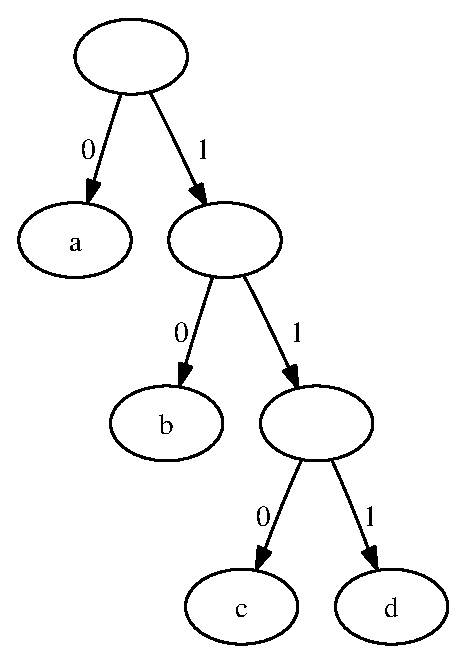
\epsfig{file=Abbildungen/coding-tree.eps, scale=0.5}} 
  \caption{Tree representation of the encoding shown in Figure \ref{tab:coding}.}
  \label{fig:coding-tree}
\end{figure}
In order to see how a bit string can be decoded using the encoding shown in Figure \ref{fig:coding-tree}
we consider the bit string ``\mytt{100111}''.  We start with the bit ``\mytt{1}'' which commands us to take
the right edge from the root of the coding tree.  Next, the bit ``\mytt{0}'' specifies the left edge.  
After following this edge we arrive at the leaf labelled with the character ``\mytt{b}''.  Hence we have
found the first character.  To decode the next character, we return to the root of the tree.  The edge labelled
``\mytt{0}'' takes us to the leaf labelled with the character ``\mytt{a}''.  Hence, we have found the
second character.  Again, we return to the root of the tree.  Now the bits ``\mytt{111}'' lead us to the
character ``\mytt{d}''.  This ends the decoding of the given bit string and we have therefore found that this
bit string encodes the string ``\mytt{bad}'', i.e.~we have
\\[0.2cm]
\hspace*{1.3cm}
``\mytt{100111}'' $\simeq$ ``\mytt{bad}''.


\section{Huffman's Algorithm}
Suppose we have been given a string $s \in \Sigma^*$ where $\Sigma$ is some alphabet.  How do we find an encoding of the letters such 
that the encoding of $s$ is as short as possible?  Huffman's algorithm answers this question.  In order 
to present this algorithm, we first define the set $\mathcal{K}$ of \blue{coding trees} by induction.
\begin{enumerate}
\item $\mytt{Leaf}(c,f) \in \mathcal{K} \quad \mbox{if $c \in \Sigma$ and $f \in \N$}$.

      An expression of the form $\mytt{Leaf}(c,f)$ represent a leaf in a coding tree.  Here  $c$ is a letter
      from the alphabet $\Sigma$ and $f$ is the number of times that the letter $c$ occurs in the string $s$
      that is to be encoded.

      Compared to Figure \ref{fig:coding-tree} this representation adds the frequency $f$ of the letters.
      This frequency information is needed since we intend to code frequent letters with fewer bits.
\item $\mytt{Node}(l,r) \in \mathcal{K} \quad \mbox{if $l \in\mathcal{K}$ and $r \in \mathcal{K}$.}$ 

      The expressions $\mytt{Node}(l,r)$ represent the inner nodes of the coding-tree.
\end{enumerate}
Next, we define the function
\\[0.2cm]
\hspace*{1.3cm}
$\mytt{count} : \mathcal{K} \rightarrow \N$.
\\[0.2cm] 
This function computes the sum of all frequencies of all letters occurring in a given coding tree.
\begin{enumerate}
\item For a leaf, the definition of $\mytt{count}$ is obvious:
      \\[0.2cm]
      \hspace*{1.3cm}
      $\mytt{Leaf}(c,f).\mytt{count}() = f$.
\item The sum of all frequencies of a coding tree of the form $\mytt{Node}(l,r)$ is the sum of all frequencies
      in $l$ plus the frequencies in $r$.  Therefore we have
      \\[0.2cm]
      \hspace*{1.3cm}
      $\mytt{Node}(l,r).\mytt{count}() = l.\mytt{count}() + r.\mytt{count}()$. 
\end{enumerate}
Next we define the function
\\[0.2cm]
\hspace*{1.3cm}
$\mytt{cost}: \mathcal{K} \rightarrow \N$.
\\[0.2cm]
The function $\mytt{cost}$ computes the number of bits that are necessary to encode a string $s$ if 
all letters occurring in $s$ occur in the the coding tree and if, furthermore, the frequencies of the letters
in $s$ are given by the frequencies stored in the coding tree.
The definition of $\mytt{cost}(t)$ is given by induction on the coding tree $t$.
\begin{enumerate}
\item $\mytt{Leaf}(c,f).\mytt{cost}() = 0$.

      As long as the coding tree has no edges, the resulting encoding has zero bits.
\item $\mytt{Node}(l,r).\mytt{cost}() = 
       l.\mytt{cost}() + r.\mytt{cost}() + l.\mytt{count}() + r.\mytt{count}()$.

      If two coding trees $l$ and $r$ are combined into a new coding tree, the encoding of all letters
      occurring in either $l$ or $r$ grows by one bit:  The encoding of a letter in $l$ is prefixed with the
      bit ``$0$'', while the encoding of a letter from $r$ is prefixed with the bit ``$1$''.  The sum
      \\[0.2cm]
      \hspace*{1.3cm}
      $l.\mytt{count}() + r.\mytt{count}()$
      \\[0.2cm] 
      counts the frequencies of all letters occurring in the coding tree.
      As the encoding of all these letters is lengthened by one bit,
      we have to add the term $l.\mytt{count}() + r.\mytt{count}()$ to the costs of $l$ and $r$.
\end{enumerate}
The function  $\mytt{cost}()$ is extended to sets of coding trees.  If $M$ is a set of coding trees, then we
define
\\[0.2cm]
\hspace*{1.3cm}
$\mytt{cost}(M) := \sum\limits_{n\in M} n.\mytt{cost}()$. 
\\[0.2cm]
The algorithm that was published by David A.~Huffman in 1952 \cite{huffman:52} starts with a set of pairs of
the form $\langle c, f\rangle$ where $c$ is a letter and $f$ is the frequency of this letter on a given string
$s$ that is to be encoded.  In the first step of this algorithm, these pairs are turned into leaves of a coding tree.
Assume that the string $s$ is built from the  letters
\\[0.2cm]
\hspace*{1.3cm}
$c_1$, $c_2$, $\cdots$, $c_k$
\\[0.2cm]
and that the frequencies of theses letters are givens as
\\[0.2cm]
\hspace*{1.3cm}
$f_1$, $f_2$, $\cdots$, $f_k$.
\\[0.2cm]
Then the set of coding trees is given as
\begin{equation}
  \label{eq:huffmann1}
 M = \bigl\{  \mytt{Leaf}(c_1, f_1), \cdots, \mytt{Leaf}(c_k, f_k) \bigr\}.   
\end{equation}
Huffmann's algorithm combines two nodes $a$ and $b$ from $M$ into a new node
$\mytt{Node}(a,b)$ until the set $M$ contains just a single node.  When combining the nodes of $M$ into a single
tree we have to take care that the cost of the resulting tree should be minimal.
Huffman's algorithm takes a \href{https://en.wikipedia.org/wiki/Greedy_algorithm}{greedy} approach: 
The idea is to combine those nodes $a$ and $b$ such that the cost of the set
\\[0.2cm]
\hspace*{1.3cm}
$M \symbol{92} \{a,b\} + \{ \mytt{Node}(a,b) \}$
\\[0.2cm]
is as small as possible.
In order to choose $a$ and $b$ let us investigate how much the cost increases if we combine the two nodes
into the new node $\mytt{Node}(a,b)$:
\begin{eqnarray*}
& & \mytt{cost}\bigl(N \cup \{ \mytt{Node}(a,b) \}\bigr) - \mytt{cost}\bigl(N \cup \{ a,b \}\bigr) \\
&=& \mytt{cost}\bigl( \{ \mytt{Node}(a,b) \}\bigr) - \mytt{cost}\bigl(\{ a,b \}\bigr)              \\
&=& \mytt{Node}(a,b).\mytt{cost}() - a.\mytt{cost}() - b.\mytt{cost}()                           \\
&=&   a.\mytt{cost}() + b.\mytt{cost}() + a.\mytt{count}() + b.\mytt{count}() 
    - a.\mytt{cost}() - b.\mytt{cost}()                                                              \\
&=& a.\mytt{count}() + b.\mytt{count}() 
\end{eqnarray*}
We see that if we combine $a$ and $b$ into the new node $\mytt{Node}(a,b)$, the cost is increased by the sum 
\\[0.2cm]
\hspace*{1.3cm}
$a.\mytt{count}() + b.\mytt{count}()$. 
\\[0.2cm]
If our intention is to keep the cost small then it suggests itself to pick those nodes
$a$ and $b$ from $M$ that have the smallest count and replace them with the new node
$\mytt{Node}(a,b)$.  This process is then iterated until the set $M$ contains but a single node.
It can be shown that this procedure yields a coding tree that codes the given string using the smallest number
of bits. 

\begin{figure}[!ht]
\centering
\begin{minted}[ frame         = lines, 
                framesep      = 0.3cm,
                bgcolor       = sepia,
                numbers       = left,
                numbersep     = -0.2cm,
                xleftmargin   = 1.3cm,
                xrightmargin  = 1.3cm,
              ]{python3}
    import heapq
                  
    class CodingTree:
        pass
    
    class Leaf(CodingTree):
        def __init__(self, c, f):
            self.mCharacter = c
            self.mFrequency = f
            
        def __lt__(self, other):
            if isinstance(other, Node):
                return True
            return self.mCharacter < other.mCharacter
                
    class Node(CodingTree):
        def __init__(self, l, r):
            self.mLeft  = l
            self.mRight = r
    
        def __lt__(self, other):
            if isinstance(other, Leaf):
                return False
            return self.mLeft < other.mLeft
                
    def codingTree(M):
        H = []         # empty priority queue
        for c, f in M:
            heapq.heappush(H, (f, Leaf(c, f)))
        while len(H) > 1:
            a = heapq.heappop(H)
            b = heapq.heappop(H)
            heapq.heappush(H, (a[0] + b[0], Node(a[1], b[1])))
        return H[0][1]
\end{minted}
\vspace*{-0.3cm}
\caption{Huffman's algorithm implemented in \textsl{Python}.}
\label{fig:Huffman.ipynb}
\end{figure} 

\noindent
The function $\mytt{codingTree}$ program shown in Figure \ref{fig:Huffman.ipynb} implements this algorithm.
\begin{enumerate}
\item \textsl{Python} has a module called \mytt{heapq}.  This module implements a heap via a list.
      This module offers the following functions:
      \begin{enumerate}[(a)]
      \item Given a heap $H$ and an item $x$, the function call
            \\[0.2cm]
            \hspace*{1.3cm}
            $\mytt{heapq.heappush}(H, x)$
            \\[0.2cm]
            pushes the item $x$ onto the heap $H$.  The item $x$ serves both as a priority and a value.
            In applications of \mytt{heapq} the items are usually pairs of the form $(p, v)$ where $p$ is a
            priority (often represented as a natural number) and $v$ is some value.

            The function call $\mytt{heappush}(H, x)$ does not return a value.  Rather, the heap $H$ is
            modified in place.
      \item Given a heap $H$, the function call
            \\[0.2cm]
            \hspace*{1.3cm}
            $\mytt{heapq.heappop}(H)$
            \\[0.2cm]
            returns the object from $H$ that has the highest priority and removes this object from the heap
            $H$.
      \item As heaps are represented as lists, the empty heap is represented by the empty list.
      \end{enumerate}
\item We define a superclass \mytt{CodingTree} and two derived classes \mytt{Leaf} and \mytt{Node}.
      As we want to place objects of these classes onto a priority queue, we have to make them comparable.
      This is done by defining the method \mytt{\_\_lt\_\_} in these classes.  This method is automatically 
      called whenever two objects of class \mytt{CodingTree} are compared using the operator $<$.
      As this only happens when the corresponding counts are different, the precise implementation of this
      method does not matter as long as we take care to ensure that $<$ is a linear order.
\item The function $\mytt{codingTree}$ is called with a set  $M$ of pairs.  This set has the form
      \\[0.2cm]
      \hspace*{1.3cm}
      $M = \bigl\{ (c_1, f_1), \cdots, (c_k, f_k) \bigr\}$.
      \\[0.2cm]
      Here, $c_1$, $\cdots$, $c_k$ are the different character that occur in the string $s$ that is to be encoded. 
      For every character $c_i$, the number $f_i$ counts the number of times that $c_i$ occurs in the string
      $s$.
\item Line 27 creates the empty heap.
\item The \mytt{for}-loop in line 28 turns pairs of the form $(c, f)$ into pairs of the form
      \\[0.2cm]
      \hspace*{1.3cm}
      $\bigl(f, \mytt{Leaf}(c, f)\bigr)$
      \\[0.2cm]
      In the pairs $\bigl(f, \mytt{Leaf}(c, f)\bigr)$ the frequency $f$ is stored first because
      when \textsl{Python} compares two pairs $(x_1, y_1)$ and $(x_2, y_2)$, the comparison is done
      \blue{lexicograhically}, i.e.~we have
      \\[0.2cm]
      \hspace*{1.3cm}
      $(x_1, y_1) < (x_2, y_2)$ \quad iff \quad $x_1 < x_2 \vee (x_1 = x_2 \wedge y_1 < y_2)$.
      \\[0.2cm]
      Therefore the pair $\bigl(f_1, \mytt{Leaf}(c_1, f_1)\bigr)$ has a higher priority than the pair
      $\bigl(f_2, \mytt{Leaf}(c_2, f_2)\bigr)$ if $f_1 < f_2$.  If the frequencies $f_1$ and $f_2$ are the
      same, then the priority is decided by comparing the objects $\mytt{Leaf}(c_1, f_1)$ and
      $\mytt{Leaf}(c_2, f_2)$.  For the purpose of string compression the order does not matter in this case.

      The pairs  $\bigl(f, \mytt{Leaf}(c, f)\bigr)$ are inserted into the heap $H$.
\item The \mytt{while} loop in line 2 reduces the number of nodes of the set $M$ in every step by one.
      This is done by combining the nodes $a$ and $b$ into a single node $\mytt{Node}(a, b)$
      \begin{enumerate}
      \item Using the function $\mytt{heappop}$ we compute those nodes $a$ and $b$ that have the lowest 
            character count and remove them from the heap $H$.
      \item Next $a$ and $b$ are combined into the new node $\mytt{Node}(a,b)$ that is added to $H$.
      \end{enumerate}
\item The \mytt{while} loop terminates when $H$ contains but a single element.  This element
      is then returned as the result.
\end{enumerate}
The running time of Huffman's algorithm is given as  $\Oh\bigl(n \cdot \ln(n)\bigr)$ where $n$ denotes the
number of different characters occurring in the string $s$.  The reason is that all
the operations inside the \mytt{while} loop have at most a logarithmic complexity in $n$ and the loop is
executed $n-1$ times.
 

\begin{table}[htbp]
  \centering
\begin{tabular}[t]{|l|r|r|r|r|r|}
\hline
Character  & \mytt{a} & \mytt{b} & \mytt{c} & \mytt{d} & \mytt{e} \\
\hline
\hline
Frequency &          1 &          2 &          3 &          4 &          5 \\
\hline
\end{tabular}
  \caption{Letters with their frequencies.}
  \label{tab:frequency}
\end{table}

We demonstrate Huffman's algorithm by computing  the coding tree that results from a string $s$ containing the
letters ``\mytt{a}'', ``\mytt{b}'', ``\mytt{c}'', ``\mytt{d}'', and ``\mytt{e}'' where the number of
occurrence of these letters are given in table \ref{tab:frequency} on page \pageref{tab:frequency}.
\begin{enumerate}
\item Initially, the set $M$ has the form
      \\[0.2cm]
      \hspace*{0.3cm}
      $ M = \bigl\{ \langle 1, \mytt{Leaf}(\mytt{a}) \rangle,\,
             \langle 2, \mytt{Leaf}(\mytt{b}) \rangle,\, 
             \langle 3, \mytt{Leaf}(\mytt{c}) \rangle,\,
             \langle 4, \mytt{Leaf}(\mytt{d}) \rangle,\,
             \langle 5, \mytt{Leaf}(\mytt{e}) \rangle\bigr\}. $
\item Apparently, the characters ``\mytt{a}'' and ``\mytt{b}'' occur with the lowest frequency.  Hence,
  these characters are removed from $M$ and instead the node 
      \\[0.2cm]
      \hspace*{0.3cm}
      $\mytt{Node}(\mytt{Leaf}(\mytt{a}), \mytt{Leaf}(\mytt{b}))$
      \\[0.2cm]
      is added to the set $M$.  The frequency of this new node is given as the sum of the frequencies of the
      characters ``\mytt{a}'' and ``\mytt{b}''.   Hence, the pair 
      \\[0.2cm]
      \hspace*{0.3cm}
      $\langle 3, \mytt{Node}\bigl(\mytt{Leaf}(\mytt{a}) \rangle, \mytt{Leaf}(\mytt{b}) \bigr) \rangle$
      \\[0.2cm]
      is inserted into the set  $M$.  The resulting form of $M$ is
      \\[0.2cm]
      \hspace*{0.3cm}
      $ \bigl\{\langle 3, \mytt{Leaf}(\mytt{c}) \rangle,\,
			\langle 3, \mytt{Node}(\mytt{Leaf}(\mytt{a}), \mytt{Leaf}(\mytt{b}))\rangle,\,
              \langle 4, \mytt{Leaf}(\mytt{d}) \rangle,\,
             \langle 5, \mytt{Leaf}(\mytt{e}) \rangle\bigr\}. $
\item The two pairs with the smallest frequencies are now
      \\[0.2cm]
      \hspace*{0.3cm}
      $ \langle 3, \mytt{Node}(\mytt{Leaf}(\mytt{a}), \mytt{Leaf}(\mytt{b})) \rangle \quad \mathrm{and} \quad \langle 3, \mytt{Leaf}(\mytt{c})\rangle$.
      \\[0.2cm]
      These pairs are removed form $M$ and replaced by 
      \\[0.2cm]
      \hspace*{0.3cm}
      $ \langle 6, \mytt{Node}(
           \mytt{Node}((\mytt{Leaf}(\mytt{a}), \mytt{Leaf}(\mytt{b})),\; 
           \mytt{Leaf}(\mytt{c}))\rangle$. 
      \\[0.2cm]
      Then $M$ is given as
      \\[0.2cm]
      \hspace*{0.3cm}
      $ \Bigl\{ 
        \langle 4, \mytt{Leaf}(\mytt{d}) \rangle,\;\langle 5, \mytt{Leaf}(\mytt{e}) \rangle,\;
        \langle 6, \mytt{Node}(
           \mytt{Node}(\mytt{Leaf}(\mytt{a}), \mytt{Leaf}(\mytt{b})),\; 
           \mytt{Leaf}(\mytt{c}))\Bigr\}. $
\item Now the pairs
      \\[0.2cm]
      \hspace*{0.3cm}
      $ \langle 4, \mytt{Leaf}(\mytt{d}) \rangle \quad \mathrm{and} \quad \langle 5, \mytt{Leaf}(\mytt{e}) \rangle$
      \\[0.2cm]
      are the pairs with the smallest frequency.
      We remove them and construct the new node \\[0.2cm]
      \hspace*{0.3cm}
      $\langle 9, \mytt{Node}(\mytt{Leaf}(\mytt{d}), \mytt{Leaf}(\mytt{e})) \rangle$.
      \\[0.2cm]
      This node is added to the set  $M$ and then $M$ is
      \\[0.2cm]
      \hspace*{0.3cm}
      $ \Bigl\{ 
        \langle 6, \mytt{Node}(
           \mytt{Node}(\mytt{Leaf}(\mytt{a}),
           \mytt{Leaf}(\mytt{b})),\,\mytt{Leaf}(\mytt{c},3))
        \rangle,\;
        \langle 9,\mytt{Node}(\mytt{Leaf}(\mytt{d},4), \mytt{Leaf}(\mytt{e},5)) \rangle
        \Bigr\}
           $.      
\item Now the set $M$ has just two elements.  These are combined into the single node 
      \\[0.2cm]
      \hspace*{0.3cm}
      $\mytt{Node}\biggl(
              \mytt{Node}\Bigl(
                 \mytt{Node}\bigl(\mytt{Leaf}(\mytt{a}), \mytt{Leaf}(\mytt{b})\bigr),\; 
                 \mytt{Leaf}(\mytt{c})\Bigr),\;
              \mytt{Node}\bigl(\mytt{Leaf}(\mytt{d}), \mytt{Leaf}(\mytt{e})\bigr)
         \biggr)
      $.
      \\[0.2cm]
      This node is our result.  Figure 
      \ref{fig:coding-tree2} shows the corresponding coding tree.  Here every node $n$ is labelled with its
      count.  The resulting encoding is shown in table  \ref{tab:coding2}.
\end{enumerate}

\begin{figure}[!ht]
  \centering
  \framebox{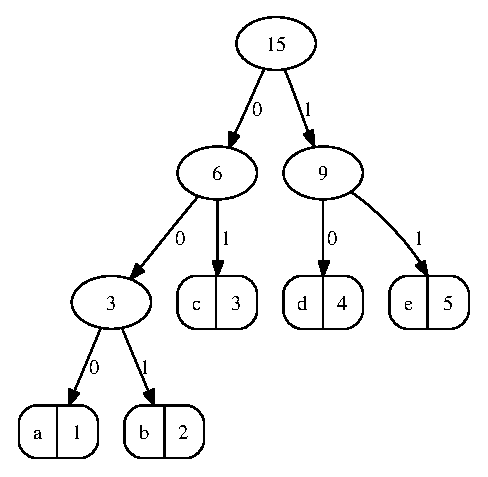
\epsfig{file=Abbildungen/coding-tree2.eps, scale=0.7}} 
  \caption{Tree representation of the coding tree.}
  \label{fig:coding-tree2}
\end{figure}



\begin{table}[htbp]
  \centering
\begin{tabular}[t]{|l|r|r|r|r|r|}
\hline
Character &   \mytt{a} &   \mytt{b} & \mytt{c}  & \mytt{d}  & \mytt{e}   \\
\hline
\hline
Encoding & \mytt{000} & \mytt{001} & \mytt{01} & \mytt{10} & \mytt{11} \\
\hline
\end{tabular}
  \caption{Variable length encoding of the letters ``\mytt{a}'' to ``\mytt{e}''.}
  \label{tab:coding2}
\end{table}
\pagebreak

\exercise
\begin{enumerate}[(a)]
\item Compute the Huffman code for a string $s$ that contains the letters 
      ``\mytt{a}'' through ``\mytt{g}'' where the frequencies are given by the following table:

\begin{table}[htbp]
  \centering
\begin{tabular}[t]{|l|r|r|r|r|r|r|r|}
\hline
Character  & \mytt{a} & \mytt{b} & \mytt{c} & \mytt{d} & \mytt{e} & \mytt{f} & \mytt{g} \\
\hline
\hline
Frequency &          1 &          1 &          2 &          3 &          5 &         8 &         13 \\
\hline
\end{tabular}
  \caption{Letters with frequencies.}
  \label{tab:aufgabe-huffman}
\end{table}

\item How many bits do we save when we use the Huffman encoding compared to a fixed with encoding?
      \eox
\end{enumerate}

\section{Check Your Understanding}
\begin{enumerate}[(a)]
\item What are the two principal ideas that can be used to compress a string?  
\item How is the set $\mathcal{K}$ of coding trees defined?
\item Define a function $\mytt{encode}: \Sigma^* \times \mathcal{K} \rightarrow \{0,1\}^*$
      that takes a string $s \in \Sigma^*$ and a coding tree $k \in \mathcal{K}$ and that produces
      a binary string $b$ that encodes the string $s$ using the coding tree $k$.
\item Define a function $\mytt{decode}:\{0,1\}^* \times \mathcal{K} \rightarrow \Sigma^*$ that takes a binary
      string $b$ and a coding tree $k$ and decodes $b$ according to the coding tree $k$.      
\item Assume you are given a dictionary $\mytt{D}$ such that for every character $c\in \Sigma$ we have that
      $D[c]$ is the number of occurrences of the character $c$ in a string $s \in \Sigma^*$.
      Are you able to implement a function \texttt{codingTree} that is able to compute the Huffman
      coding tree for this string?

      \hint
      We have implemented a similar function in this chapter.
\end{enumerate}

%%% Local Variables: 
%%% mode: latex
%%% TeX-master: "algorithms"
%%% End: 
